\documentclass[tikz,border=10pt]{standalone}
\usepackage{amsmath}
\usepackage{amssymb}
\usepackage{tikz}
\usetikzlibrary{arrows.meta,calc,decorations.pathreplacing,patterns,shapes.geometric,positioning,shadings}

\begin{document}
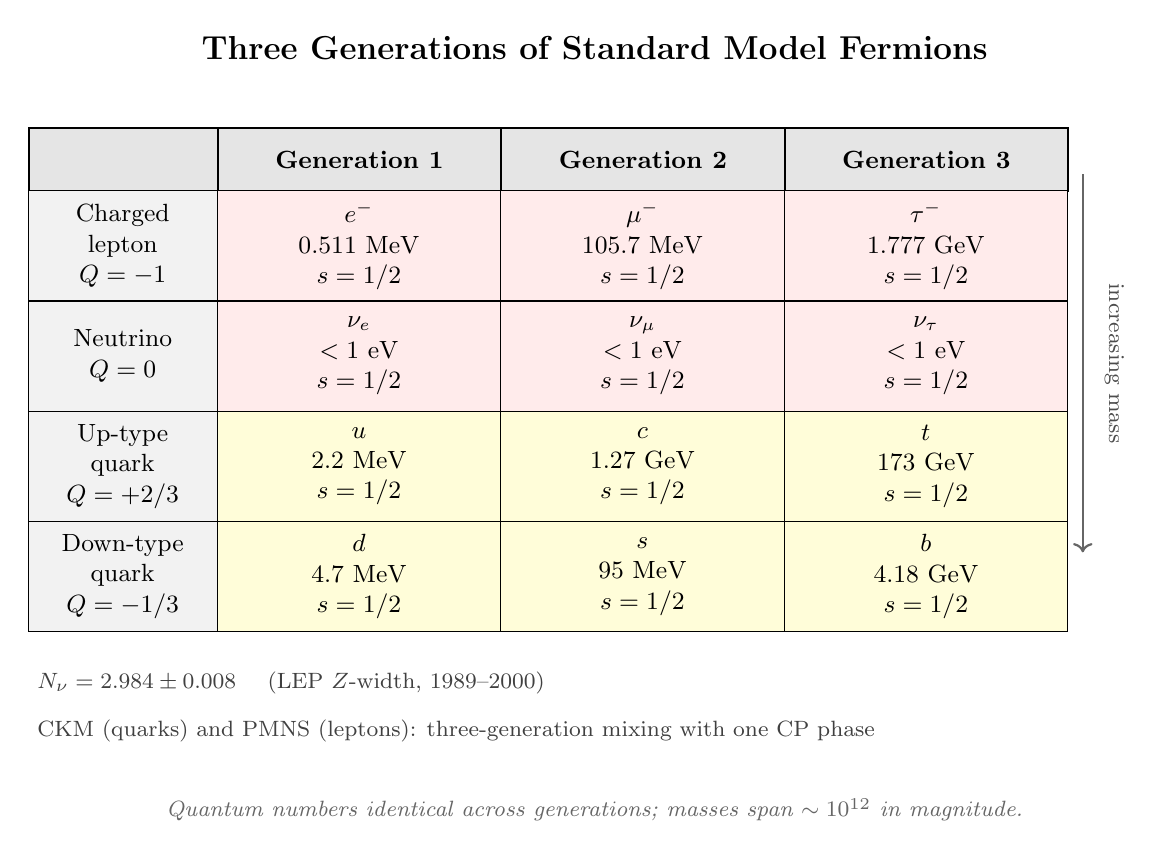
\begin{tikzpicture}[
    font=\small,
    headerstyle/.style={fill=black!10, draw=black, thick, minimum height=8mm, minimum width=36mm, inner sep=2pt},
    rowlabel/.style={fill=black!5, draw=black, thin, minimum height=14mm, minimum width=24mm, inner sep=2pt, align=center},
    leptonCell/.style={fill=red!8, draw=black, thin, minimum height=14mm, minimum width=36mm, inner sep=2pt, align=center},
    quarkCell/.style={fill=yellow!15, draw=black, thin, minimum height=14mm, minimum width=36mm, inner sep=2pt, align=center},
    smallnote/.style={font=\footnotesize, color=black!70}
]

% ============== Title ==============
\node[font=\bfseries\large] (title) at (0,0) {Three Generations of Standard Model Fermions};

% ============== Header Row ==============
\node[headerstyle, minimum width=24mm, anchor=north west] (h0) at (-72mm, -10mm) {};
\node[headerstyle, anchor=north west] (h1) at (-48mm, -10mm) {\textbf{Generation 1}};
\node[headerstyle, anchor=north west] (h2) at (-12mm, -10mm) {\textbf{Generation 2}};
\node[headerstyle, anchor=north west] (h3) at (24mm, -10mm) {\textbf{Generation 3}};

% ============== Row 1: Charged Leptons ==============
\node[rowlabel, anchor=north west, minimum height=14mm] (lblL) at (-72mm, -18mm) {Charged\\lepton\\$Q=-1$};
\node[leptonCell, anchor=north west] (L1) at (-48mm, -18mm) {$e^-$ \\ $0.511$ MeV \\ $s=1/2$};
\node[leptonCell, anchor=north west] (L2) at (-12mm, -18mm) {$\mu^-$ \\ $105.7$ MeV \\ $s=1/2$};
\node[leptonCell, anchor=north west] (L3) at (24mm, -18mm) {$\tau^-$ \\ $1.777$ GeV \\ $s=1/2$};

% ============== Row 2: Neutrinos ==============
\node[rowlabel, anchor=north west, minimum height=14mm] (lblN) at (-72mm, -32mm) {Neutrino\\$Q=0$};
\node[leptonCell, anchor=north west] (N1) at (-48mm, -32mm) {$\nu_e$ \\ $<1$ eV \\ $s=1/2$};
\node[leptonCell, anchor=north west] (N2) at (-12mm, -32mm) {$\nu_\mu$ \\ $<1$ eV \\ $s=1/2$};
\node[leptonCell, anchor=north west] (N3) at (24mm, -32mm) {$\nu_\tau$ \\ $<1$ eV \\ $s=1/2$};

% ============== Row 3: Up-type Quarks ==============
\node[rowlabel, anchor=north west, minimum height=14mm] (lblU) at (-72mm, -46mm) {Up-type\\quark\\$Q=+2/3$};
\node[quarkCell, anchor=north west] (U1) at (-48mm, -46mm) {$u$ \\ $2.2$ MeV \\ $s=1/2$};
\node[quarkCell, anchor=north west] (U2) at (-12mm, -46mm) {$c$ \\ $1.27$ GeV \\ $s=1/2$};
\node[quarkCell, anchor=north west] (U3) at (24mm, -46mm) {$t$ \\ $173$ GeV \\ $s=1/2$};

% ============== Row 4: Down-type Quarks ==============
\node[rowlabel, anchor=north west, minimum height=14mm] (lblD) at (-72mm, -60mm) {Down-type\\quark\\$Q=-1/3$};
\node[quarkCell, anchor=north west] (D1) at (-48mm, -60mm) {$d$ \\ $4.7$ MeV \\ $s=1/2$};
\node[quarkCell, anchor=north west] (D2) at (-12mm, -60mm) {$s$ \\ $95$ MeV \\ $s=1/2$};
\node[quarkCell, anchor=north west] (D3) at (24mm, -60mm) {$b$ \\ $4.18$ GeV \\ $s=1/2$};

% ============== Bottom annotations ==============
\node[anchor=north west, font=\footnotesize, color=black!75] at (-72mm, -78mm)
    {$N_\nu = 2.984 \pm 0.008$ \quad (LEP $Z$-width, 1989--2000)};
\node[anchor=north west, font=\footnotesize, color=black!75] at (-72mm, -84mm)
    {CKM (quarks) and PMNS (leptons): three-generation mixing with one CP phase};

% ============== Mass-hierarchy arrows on the right ==============
\draw[->, thick, black!60] (62mm, -16mm) -- (62mm, -64mm);
\node[rotate=-90, font=\footnotesize, color=black!70] at (66mm, -40mm) {increasing mass};

% ============== Footnote ==============
\node[font=\footnotesize\itshape, color=black!60, anchor=north] at (0mm, -94mm)
    {Quantum numbers identical across generations; masses span $\sim 10^{12}$ in magnitude.};

\end{tikzpicture}
\end{document}
